\begin{figure*}
  \begin{center}
    \begin{tabular}{c}
      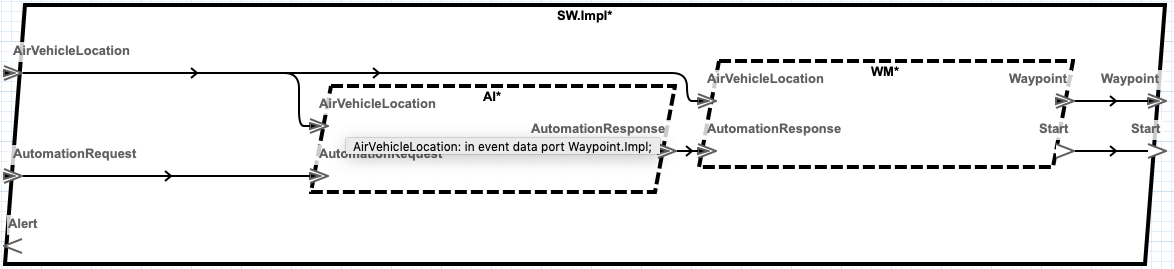
\includegraphics[scale=0.4]{example.png} \\
      (a) \\
      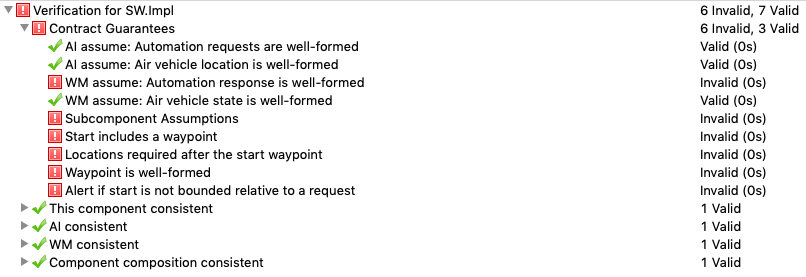
\includegraphics[scale=0.4]{example-certificate.png} \\
      (b)
    \end{tabular}
  \end{center}
\caption{Automated UAV route planning system. (a) Unhardened system. (b) Failure certificate.}
\label{fig:example}
\end{figure*}

\figref{fig:example} is an AADL description of an implementation of a software system for route planning and automated control for a UAV. It is loosely based on the system in the case study presented later. The system receives an automation request that is forwarded to an untrusted third-party route planner (AI) that decides the flight path of the UAV based on its current position and the requested task. The waypoint manager (WM) receives the mission command as a set of waypoints from the planner and starts the UAV flying the mission, issuing waypoints to the UAV flight control as the UAV location changes. It is a legacy component that is not subject to change. The alert manager never raises the alert as there is no capacity in the initial design to know when an alert is needed.

The goal is to cyber-harden the system so that it is resilient to cyber-attack. For this simple example, two attacks are considered, both originating from the untrusted route-planner: first, malformed messages to disrupt the waypoint manager or UAV flight control; and second, a delayed or unrequested automation response to prevent the UAV from flying a mission or to fly the wrong mission.

\begin{figure}
  \begin{center}
    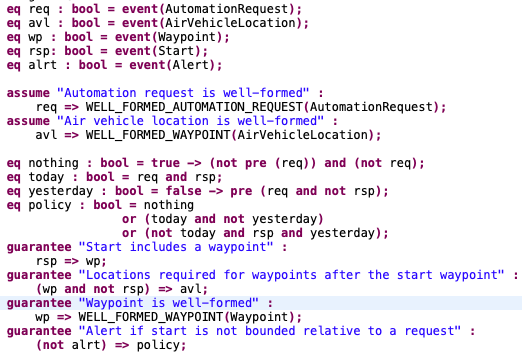
\includegraphics[scale=0.4]{sw.png}
  \end{center}
  \caption{The SW component contract.}
  \label{fig:sw}
\end{figure}

This work uses an assume guarantee paradigm, in the form of contracts, to model and hierarchically prove properties of the system (cite AGREE). The contracts constrain the inputs and state properties output for component models. In this example, the model for the route planner assumes its input is well-formed, but it makes no guarantees about its output as it is an untrusted third party component. The contract for the legacy waypoint manager makes similar assumptions about its input, but unlike the route planner, the model constrains its output to be well-formed and coincide with the mission command from the route planner and the air vehicle location.\footnote{See (cite repository) for the full model with contracts.}

The contract to model the SW component with its primary inputs and outputs is in \figref{fig:sw}. The contract language is a first order predicate calculus. The contract semantics are synchronous data-flow where the inputs, outputs, and expressions are characterized by data streams. The semantics are such that the contracts are evaluated in dependency order with inputs being propagated to outputs through all the contracts until they stabilize; as such, the contracts, and thereby the system model, must be acyclic. Once the contracts have stabilized, then the model takes a synchronous step to the next input data in the stream.  

The contract in \figref{fig:sw} uses \texttt{eq} statements to define variables local to the contract. For example, the \texttt{req} variable is equivalent to the \texttt{event(req)} expression. An \texttt{event} expression is true if there is data on the named AADL event port. The system contract assumes well-formed input and guarantees a set of properties about the output.

There are two requirements in the SW model, among others, related to the cyber-attacks: the first, \emph{Waypoint is well-formed} disallows malformed waypoints from being propagated; the second, \emph{Alert if start is not bounded relative to a request}, disallows a mission being started without a request or if the start is delayed more than one step after a request. This later guarantee merits some further discussion as it illustrates the steam nature of the semantics.

The guarantee is an invariant on the expression \texttt{not alrt => policy} meaning that if there is not an alert output then the policy must hold (and if there is an alert, then the policy does not matter). The \texttt{policy} is satisfied if there is no pending request (\texttt{nothing}), a request with a response right now (\texttt{today}), or a request yesterday with its response today. 

The expression for \texttt{yesterday} is helpful to understanding data streams and the synchronous data-flow semantics. It uses the \texttt{->} operator for initialization. The left operand is the initial value of \texttt{yesterday} at the start of the system, which in this example is \texttt{false} because there is no yesterday at the start.  The right operand is the value of \texttt{yesterday} after the initial step. Here the stream nature of expressions is apparent with the \texttt{pre} operator referring to the value of \texttt{(req and not rsp)} in the prior time step. Intuitively, \texttt{yesterday} is true if the previous time step made a request without a matching response. The \emph{Alert if start is not bounded relative to a request} defines the behavior of the correctly implemented system which is that it alerts if the bounded response policy does not hold. In this way, the contracts model the expected input and output of the system as a whole and also between components that implement the system.

Model checking proves whether the contract models of the components, with their connections, implement the system model in \figref{fig:sw}. The results of the model checker are in \figref{fig:example}(b). Not unexpectedly, since the model of the route planner leaves the output behavior unconstrained (i.e., the component can do anything since it is not trusted) the model checker proves that the component composition does not implement the system requirements.

\begin{figure*}
  \begin{center}
    \begin{tabular}{c}
      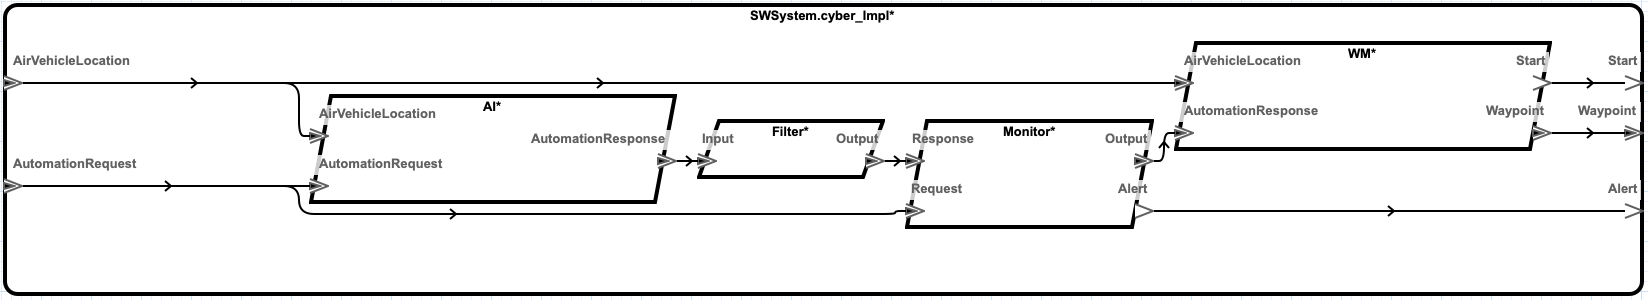
\includegraphics[scale=0.3]{hardened.png} \\
      (a) \\
      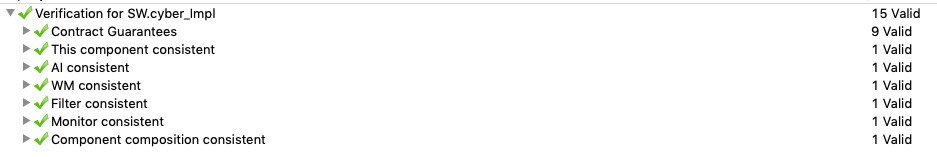
\includegraphics[scale=0.4]{hardened-certificate.png} \\
      (b)
    \end{tabular}
  \end{center}
  \caption{Hardened UAV system. (a) The implementation with high-assurance components. (b) Passing certificate.}
  \label{fig:hardened}
\end{figure*}

\begin{figure}
  \begin{center}
    \begin{tabular}{c}
      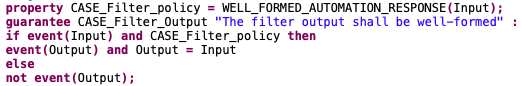
\includegraphics[scale=0.45]{filter.png} \\
      (a) \\
      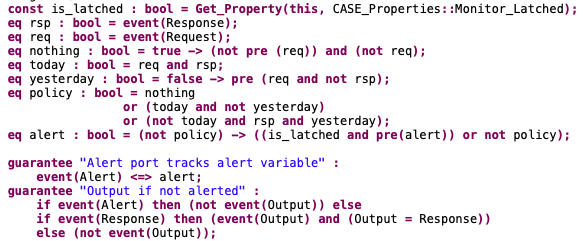
\includegraphics[scale=0.4]{monitor.png} \\
      (b)
    \end{tabular}
  \end{center}
  \caption{High-assurance component contracts. (a) The filter. (b) The monitor.}
  \label{fig:assurance}
\end{figure}

The system implementation is cyber-hardened by inserting high-assurance components in the form of a filter and a monitor as shown in \figref{fig:hardened}(a). A filter takes a stream of data and delivers a new stream of data where some property is enforced. Its stylized form generated by the CASE tools is shown in \figref{fig:assurance}(a). The user must provide the meaning of the property, a predicate, while the tool generates everything else. In this example, the property is the assumption made by the waypoint manager about the automation response being well-formed. The guarantee is such that it has a trivial direct mapping to synthesized code by completely specifying the behavior of the output.

A monitor captures a relation over time on data and is able to reason about temporal properties. In this example, the monitor only forwards responses that meet the bounded response property as shown in \figref{fig:assurance}(b). Like the filter, the generated monitor, with its contract, is stylized for synthesis only requiring the user to indicate the policy and some extra information for the output. The policy is taken from the contract in \figref{fig:sw} since it is the monitor that needs to alert violations of the bounded response.

The proof certificate for the new cyber-hardened implementation is in \figref{fig:hardened}(b). The high-assurance components guarantee the correct behavior of the SW implementation in the presence of the considered cyber attacks.

The high-assurance components are automatically synthesized from the contract models for the final deployed system. Synthesis assumes the existence of the communication fabric and a scheduler that implements the synchronous data-flow semantics by dispatching components in dependency order. For this example, and the later case study, the HAMR framework provides both requirements.

\newsavebox{\boxa}
\begin{lrbox}{\boxa}
\begin{lstlisting}
fun filter_step () =
let val () = Utils.clear_buf filterBuffer
    val () = API.callFFI "get_input" "" filterBuffer
    val string = Utils.buf2string filterBuffer
in
    if WELL_FORMED_AUTOMATION_RESPONSE string
    then
        let val string = Word8Array.substring filterBuffer 1
                         (Word8Array.length filterBuffer - 1)
        in API.callFFI "put_output" string Utils.emptybuf
        end
    else print"Filter rejects message.\n"
end
\end{lstlisting}
\end{lrbox}

\begin{figure}
  \begin{center}
    \begin{tabular}{c}
      \scalebox{0.60}{\usebox{\boxa}}
    \end{tabular}
  \end{center}
  \caption{Synthesized CakeML for the filter.}
  \label{fig:cakeml}
\end{figure}

Synthesis targets CakeML, and CakeML provides verified compilation to binaries for several different platforms. The generated code for the filter is shown in \figref{fig:cakeml}. The code is called at dispatch by the scheduler. The \texttt{API.callFFI} is the link to the communication fabric to capture input. The body of the function restates the filter contract to make the appropriate assignments in a way that matches the truth value of the predicate. The synthesis is proven to exactly implement the meaning of the contract in the synchronous data-flow semantics in the CakeML assuming perfect communication and scheduling.
